%!TEX program = pdflatex

\documentclass[11pt, landscape, a4paper]{article}
\usepackage{geometry}[landscape]
\usepackage{multicol}
\usepackage{graphicx}
\usepackage{amsmath} 
\usepackage{amssymb}
\usepackage[unicode]{hyperref}

\usepackage[dvipsnames]{xcolor}
\usepackage{mathptmx}
\usepackage[compact]{titlesec}
\usepackage{paralist}
\usepackage{mathtools}

\usepackage{tabularx}
\usepackage{ctable}
\usepackage[inline]{enumitem}

% Set page margins
\geometry{top=.5cm, left=.5cm, right=.5cm, bottom=.5cm}

% Set indentation
\setlength{\parindent}{0pt}
\setlength{\parskip}{0cm}

% Set path for assets
\graphicspath{{assets/}}

\setlength{\columnsep}{5pt}
\raggedcolumns

% _____ CUSTOM COMMANDS __________________________________________
\newcommand{\E}[0]{\mathbb{E}}
\newcommand{\N}[0]{\mathbb{N}}
\newcommand{\R}[0]{\mathbb{R}}

\newcommand{\sgn}[0]{\text{sgn}}

\newcommand{\argmin}[1]{\underset{#1}{\text{argmin}}}
\newcommand{\argmax}[1]{\underset{#1}{\text{argmax}}}

\titlespacing{\section}{0pt}{0.3ex}{0ex}
\titlespacing{\subsection}{0pt}{0ex}{0ex}
\linespread{0.7}

\newcommand*{\myfont}{\fontfamily{phv}\selectfont}

\titleformat*{\section}{\myfont\bfseries\color{cyan}}
\titleformat*{\subsection}{\myfont\bfseries\color{magenta}}

\begin{document}
\begin{multicols*}{4}

\setlength{\abovedisplayskip}{0pt}
\setlength{\belowdisplayskip}{0pt}
\setlength{\abovedisplayshortskip}{0pt}
\setlength{\belowdisplayshortskip}{0pt}

\newcommand{\middot}{~\textperiodcentered~}
\newlist{rowlist}{enumerate*}{1}
\setlist[rowlist]{label={\textbf{\roman*}\text{: }}, afterlabel={}, itemjoin=\middot}


% _____ CONTENT __________________________________________________

% main heading
%\begin{center}
%	\Large{\te xtbf{Introduction to ML}} \\
%    \small{by dcamenisch}
%\end{center}

\section*{Model Error}

\textbf{Empirical Risk} \quad \ $\hat R_D(f) = \frac{1}{n} \sum \mathcal \ell(y, f(x))$

\textbf{Population Risk} \quad $R(f) = \E_{x,y \sim p}[\ell(y, f(x))]$

It holds that $\E_D[\hat R_D (\hat f)] \leq R(\hat f)$. We call $R(\hat f)$ the generalization error. Expected estimation error is $\E_{X}\ell(f(X), f^\ast(X))$.

\textbf{Bias Variance Tradeoff}:

Pred. error = \color{red} Bias$^2$ \color{black} + \color{blue} Variance \color{black} + \color{ForestGreen} Noise \color{black}
\begin{align*}
	\E_D[R(\hat f)] &= \color{red} \E_x[f^*(x) - \E_D[\hat f_D(x)]]^2 \\[-4pt]
 	&+ \color{blue} \E_x[\E_D[(\hat f_D(x) - \E_D[\hat f_D(x)])^2]] \color{black}  + \color{ForestGreen} \sigma
\end{align*}

\textbf{Bias}: how close $\hat f$ can get to $f^*$

\textbf{Variance}: how much $\hat f$ changes with $D$

\section*{Regression}

\textbf{Squared loss} \quad (convex)

\qquad \qquad $\frac{1}{n}\sum (y_i - f(x_i))^2 = \frac{1}{n}||y - X w||_2^2$

\qquad \qquad $\nabla_w L(w) = 2X^\top(Xw -y)$

Solution: $\hat{w} = (X^\top X)^{-1}X^\top y$

\subsection*{Regularization}

\textbf{Lasso Regression} \quad (sparse)

\qquad \qquad $\argmin{w \in \R^d} ||y - \Phi w||_2^2 + \lambda ||w||_1$

\textbf{Ridge Regression}

\qquad \qquad $\argmin{w \in \R^d} ||y - \Phi w||_2^2 + \lambda ||w||_2^2$

\qquad \qquad $\nabla_w L(w) = 2X^\top(Xw -y) + 2 \lambda w$

Solution: $\hat w = (X^\top X + \lambda I)^{-1} X^\top y$

large $\lambda \Rightarrow$ larger bias but smaller variance 

\subsection*{Standardization}
Goal: each feature: $\mu = 0$, unit $\sigma^2$: $\tilde{x}_{i,j} = \frac{(x_{i,j}-\hat{\mu}_j)}{\hat{\sigma}_j}$\\
$\hat{\mu}_j = \frac{1}{n}\sum_{i=1}^n x_{i,j}$, $\hat{\sigma}_j^2 = \frac{1}{n}\sum_{i=1}^n {(x_{i,j}-\hat{\mu}_j)}^2$ 

\subsection*{Cross-Validation}

\begin{rowlist}
	\item For all folds $i = 1,..., k$:  Train $\hat{f}_i$ on $D' - D'_i$; Val. error $R_i = \frac{1}{|D'_i|} \sum \ell(\hat{f}_i(x), y)$
	\item Compute CV error $\frac{1}{k} \sum_{i=1}^k R_i$
	\item Pick model with lowest $CV$ error
\end{rowlist}
\section*{Gradient Descent}
Converges only for convex case.
\[
	w^{t+1} = w^t - \eta_t \cdot \nabla \ell(w^t)
\]

For linear regression:
\[
	||w^t - w^*||_2 \leq ||I - \eta X^\top X||_{op}^t ||w^0 - w^*||_2
\]

$\rho = ||I - \eta X^\top X||_{op}^t$ conv. speed for const. $\eta$. Opt. fixed $\eta = \frac{2}
{\lambda_{\text{min}} + \lambda_{\text{max}}}$ and max. $\eta \leq \frac{2}{\lambda_{\text{max}}}$. 
$\lambda ~\text{from eigenv. decomp.} ~ V(I - \eta \Sigma^\top \Sigma)V^\top$

\textbf{Momentum}: $w^{t+1} = w^t + \gamma \Delta w^{t-1} - \eta_t \nabla \ell(w^t)$

\textbf{SGD}: pick point u.a.r.
\textbf{Minibatch SGD}: pick a batch u.a.r., same in expectation
\section*{Classification}

\textbf{Zero-One loss} \quad not convex nor continuous

\qquad \qquad $\ell_{0-1}(\hat{f}(x), y) = \mathbb{I}_{y \neq \sgn \hat{f}(x)}$

\textbf{Logistic loss} \quad $\log(1 + e^{-y \hat{f}(x)})$

\textbf{Hinge loss} \quad \ $\max(0, 1-y \hat{f}(x))$

\textbf{Softmax} $p(1 | x) = \frac{1}{1 + e^{- \hat{f}(x)}}, p(-1 | x) = \frac{1}{1 + e^{\hat{f}(x)}}$ 

Cross-Entropy \ \ \ $\hat{p}_k = e^{\hat{f}_k(x)} / \sum_{i=1}^K e^{\hat{f}_j(x)}$

\subsection*{Linear Classifiers}

Dec. bound: $f(x) = w^\top x + b  = 0$

If data is lin. sep. GD  converges to \textbf{Maximum-Margin Solution}: 

$w_{\text{MM}} = \text{argmax} \; \underbrace{\text{min}_i y_i w^\top x_i (w)}_{\text{margin}(w)} \; \text{, } ||w||_2 = 1$ \\[-15pt]
 
\subsection*{SVMs}
 
\textbf{\textcolor{purple}{Soft SVM} / Hard SVM} \quad \textcolor{purple}{"slack"} 
$$\hat{w} = \min_{w, \xi} \frac{1}{2} ||w||_2^2 \textcolor{purple}{ + \lambda \sum_{i=1}^n \underbrace{\max (0, 1 - y_i w^\top x_i)}_{\text{hinge loss}}}$$ \\[-10pt]
$\text{s.t. } \forall i \;y_i w^\top x_i \geq 1 \textcolor{purple}{- \xi}$ 

\subsection*{Metrics} 
$\textbf{error}_1 / \textbf{FPR}: \frac{\text{FP}}{\text{TN + FP}}$
$\textbf{error}_2 / \text{FNR}: \frac{\text{FN}}{\text{TP + FN}}$
$\textbf{TPR / Recall}: \frac{\text{TP}}{\text{TP + FN}}$
$\textbf{TNR}: \frac{\text{TN}}{\text{TN + FP}}$
$\text{Precision}: \frac{\text{TP}}{\text{TP + FP}} = 1 - \text{FDR}$, FDR = $\frac{FP}{TP + FP}$

\textbf{AUROC}: TPR (y) vs. FPR (x)

\textbf{F1-Score}: $\frac{2TP}{2TP+FP+FN}=\frac{2}{1/Precision+1/Recall}$, $\text{Accuracy}: \frac{\text{TP + TN}}{\text{P + N}} = \frac{TP + TN}{TP + TN + FP + FN}$

Goal: large recall and small FPR.

\section*{Kernels}

$w = \Phi^\top \alpha$ (param.ized), $k(x,y) = \varphi(x)^\top \varphi(y)$


\textbf{Valid} ~ \begin{rowlist}
    \item $K$ is sym.: $k(x,z) = k(z,x)$
    \item psd: $z^\top K z \geq 0$
    $K(x, x') = \begin{bsmallmatrix}
                k(x, x) & k(x, x') \\
                k(x', x) & k(x', x')
                \end{bsmallmatrix}$   
\end{rowlist}

find k(x, x) $<$ 0, one can prove Det(K) $<$ 0

\textbf{all monomial kernels \textcolor{purple}{up to}/\textcolor{green}{of} deg. m}: $k(x,y) = (\textcolor{purple}{1 + }x^\top y)^m$ with $\binom{d+m\textcolor{green}{-1}}{m}$ monomials

\textbf{RBF}: $k(x, z) = \exp ( -\frac{||x - z||_\alpha}{\tau} )$, $\uparrow \tau : \uparrow \text{std}$

Laplacian: $\alpha = 1$, Gaussian: $\alpha = 2$ 


\textbf{Mercers Theorem}: Valid kernels can be decomposed into a lin. comb. of inner products.

\textbf{Kernel composition}

\begin{rowlist}
    \item $\forall c > 0. \; k = c \cdot k_1$
    \item $f(k)$, where $f$ is a polynomial/power series with non-negative coefficients
    \item{
        $k(\binom{x}{y}, \binom{x'}{y'})=k(x,x')k(y,y')$, $k(\binom{x}{y}, \binom{x'}{y'})=k(x,x') + k(y,y')$ where $\binom{x}{y}$ is concatenation of vectors
    }
    \item iff. for $g$ all Taylor coefficients non-negative, then $k(x, x') = g(\left< x, x' \right>)$ is a valid kernel
    \item $\forall f. \; k(x,y) = f(x)k_1(x,y)f(y)$
\end{rowlist}

\textbf{Kern. Ridge Reg.}
Ansatz: $w^*=\Phi^\top\alpha$\\
$\min_w \frac1n \|y - \Phi w\|^2 + \lambda ||w||_2^2 = \min_\alpha \frac1n ||y - K\alpha||_2^2 + \lambda \alpha^\top K \alpha$

$\text{non-empty data, } \& \exists \hat{\alpha} : \hat{w} = \sum_{i=1}^{n} \hat{\alpha}_i \phi(x_i).$

\section*{KNN Classification}

\begin{rowlist}
	\item Pick $k$ and distance metric $d$
	\item For given $x$, find among $x_1,...,x_n \in D$ the $k$ closest to $x \to x_{i_1},..., x_{i_k}$
	\item Output the majority vote of labels
\end{rowlist}

\section*{Neural Networks}

$F(x)=W^{L}\phi^{L-1}(W^{L-1}...(\phi^{1}(W^{1}x)...))$

$\textbf{ReLU: } \max (0,z), \; \textbf{Tanh: } \frac{\exp(z) - \exp(-z)}{\exp(z) + \exp(-z)}$ \\[-3pt]
$\textbf{Sigmoid: } \varphi(z) = \frac{1}{1 + \exp(-z)}, \varphi' = (1 - \varphi) \varphi$

\begin{rowlist}
    \item vanishing G.: sigm, tanh
    \item non-linear: I, ReLu for $\geq 0$ \& sigm around 0
    \item diff: all but ReLU at 0
    \item $\mu = 0$ : I, others shift to $\uparrow \mu$
    \item ReLU edgy \& tanh, sigm smooth b.

\end{rowlist}


\textbf{Universal Approximation Theorem}: We can approximate any arbitrary smooth target function, with 1+ layer with sufficient width.

\subsection*{Forward Propagation}

Input: $v^{(0)} = [x; 1]$ \quad Output: $f = W^{(L)} v^{(L-1)}$
Hidden: $z^{(l)} = W^{(l)} v^{(l-1)}, v^{(l)} = [\varphi(z^{(l)}); 1]$


\subsection*{Backpropagation}

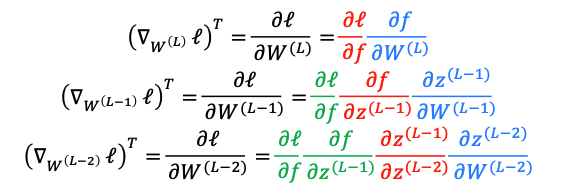
\includegraphics[width=\columnwidth]{backpropagation.png} \\[-15pt]

Weight initalization $\varphi \sim \mathcal{N}(0, \sigma)$ : $\sigma_{ReLU}=2 / n_{in}$, $\sigma_{tanh}=  1/n_{in} \text{ or } 1/ (n_{in} + n_{out})$)

\subsection*{Overfitting}
\textbf{Weight Decay} regularizes l2-norm; \textbf{Early Stopping}; \textbf{Dropout}: ignore hidden units with prob. $p$, after training use all units and scale weights by $p$; \textbf{Batch Normalization}: standardize the input in each layer

\subsection*{MLP \quad \color{Black}$\varphi(W \cdot v^{(l)}) + b$ \normalfont \textit{(fully c., ff-nn)} }
$\textbf{\#P}_{fc} = \sum_{m=1}^{L_{\text{fc}}} \left( (n_{\text{in}}^{(m)} \times n_{\text{out}}^{(m)}) + n_{\text{out}}^{(m)} \right)$


\subsection*{CNN \quad \color{Black}$\varphi(W * v^{(l)}) + b$ \normalfont \textit{(share weights, ff-nn)} }
$\textbf{\#P}_{conv} = \sum_{l=1}^{L_{\text{conv}}} \left( (k_h^{(l)} \times k_w^{(l)} \times c_{\text{in}}^{(l)} + 1) \times n_{\text{filters}}^{(l)} \right)
$
where $c_{\text{in}}^{(l)}$ =  $n_{\text{filters}}^{(l-1)}$ \& $\text{\#P}_{tot} = \text{\#P}_{conv} + \text{\#P}_{fc}$
$out_d = \frac{n_d + 2p - f_d}{s} + 1$  (ind. of \#channels)

n is input size \& f filter size of resp. d

\section*{Unsupervised Learning}

\subsection*{k-Means Clustering}

Want $\mu_i$ to minimize $\sum_{i=1}^n \min_{j\in\{1,...k\}}\|x_i-\mu_j\|_2^2$
Non-convex and NP-hard in general. Can be kernelized.

\subsection*{Lloyd's heuristic}
$\hspace*{3mm}z_i = \text{argmin}_{j\in\{1,...,k\}}\|x_i - \mu_j^{t-1}\|_2^2\\
\hspace*{3mm}\mu_j^{(t)} = \frac{1}{n_j}\sum_{i:z_i=j}x_i$\\
Monotonically decreases objective and converges to a local 
optimum. Cost per iteration $O(nkd)$, worst-case exponential

\textbf{k-Means++}: \begin{compactitem}
	\item Random data point $\mu_1 = x_i$
	\item Add $\mu_2,...,\mu_k$ rand., with prob:
		$$\text{given } \mu_{1:j} \text{ pick } \mu_{j+1} = x_i$$ 
		$\text{ where } p(i) = \frac{1}{z} \min_{l \in \{1,...,j\}} ||x_i - \mu_l||_2^2$
\end{compactitem}
Converges in expectation $\mathcal O (\log k) * \text{opt. solution}$.

\subsection*{Principal Component Analysis}

Given centered data, the PCA problem is 
$$\min_{W^\top W=I_k,z_i\in\R^k}\sum_{i=1}^n||W z_i - x_i||_2^2,$$
with solution $W^* = (v_1|...|v_k)$ where $v_i$ are the ordered 
eigvec. of $\frac{1}{n}\sum_ix_ix_i^\top$ 
and $z_i = {W^*}^\top x_i$. 

\subsection*{PCA through SVD}
\color{White} . \color {Black}\\[-10pt]
The first $k$ columns of $V$ where $X = U S V^\top$.

\subsection*{Kernel PCA}

The Kernel Principal Components are given by $\alpha^{(1)},...,\alpha^{(k)}\in \mathbb{R}^n$ 
where $\alpha^{(i)} = \frac{1}{\sqrt{\lambda_i}}v_i$ and 
$K = \sum_{i=1}^n \lambda_i v_i v_i^\top$ with ordered $\lambda_i.$ A point 
$x$ is projected to $z \in \mathbb{R}^k$:
$z_i = \sum_{j=1}^n\alpha_j^{(i)}k(x,x_j)$

\subsection*{Autoencoders}

We want to minimize $\frac{1}{n}\sum_{i=1}^n ||x_i - \hat{x}_i||_2^2$.
$$\hat{x} = f_{dec}(f_{enc}(x, \theta_{enc}); \theta_{dec})$$

Lin. activation func. \& square loss $=>$ PCA
\section*{Probabilistic Methods}

Assume $\mathcal{D} = \left\{ (x_i, y_i) \right\}_{i=1}^{n}.$ is i.i.d: $\mathbb{P}_{\mathcal{D}} = \prod_{i=1}^{n} \mathbb{P}_{X_i, Y_i}
$, 
Parametric Family: $\mathbb{P}^* = \mathbb{P}^{\theta*} \in \mathcal{P}.$  ,e.g. $\mathcal{P} = \left\{ \mathcal{N}(\mu, \sigma^2) \mid (\mu, \sigma) \in \mathbb{R}^2 \right\}.$

\subsection*{Statistical Inference}

\textbf{frequentist:} $\mathbb{P}^* \in \mathcal{P} = \left\{ \mathbb{P}; \theta; \theta \in \Theta \right\}$
\textbf{Baysian:} $\mathbb{P}^* = \mathbb{P}_{\cdot \mid \theta} \text{ with } \theta \sim \mathbb{P}_{\theta} \text{ (prior)}$ \\[-15pt]

\[
\underbrace{p( \theta \mid \mathcal{D})}_{\text{posterior}} = \underbrace{p(\mathcal{D} \mid \theta)}_{\text{likelihood}} \underbrace{p(\theta)}_{\text{prior}} / {\underbrace{p(\mathcal{D})}_{\text{evidence}}}
\] 
evidence: $p(\mathcal{D}) = \int p(\mathcal{D} \mid \theta) p(\theta) d\theta$

\subsection*{MLE \quad \color{black}$\arg \max_{\theta \in \Theta} p(\mathcal{D}; \theta)$} 
$\hat{\theta}_{\text{MLE}} \overset{\text{i.i.d.}}{:=} \arg \max_{\theta \in \Theta} \prod_{i=1}^{n} p(x_i; \theta) $

$\overset{\text{(discr.)}}{=} \frac{\partial}{\partial \theta}
 \sum_{i=1}^{n} -\log p(x_i \mid \theta) \overset{!}{=} 0$

\subsection*{MAP \quad \color{black}$\arg \max_{\theta \in \Theta} p(\theta \mid \mathcal{D})$}
$\hat{\theta}_{\text{MAP}} \overset{\text{i.i.d.}}{:=} \arg \max_{\theta \in \Theta} \left( \prod_{i=1}^{n} p(x_i\mid \theta) \right) p(\theta)$

$\overset{\text{discr.}}{=}  \frac{\partial}{\partial \theta} \sum_{i=1}^{n} -\log p(x_i \mid \theta) - \log p(\theta) \overset{!}{=} 0$ 

$\rightarrow$ MLE = MAP iff $p(\theta) \sim U$



\section*{Bayes Optimal Predictors}

Opt dec rule $f^* \text{ knowing } \mathbb{P}(Y \mid X=x)$:
$f^*(x) := \arg \min_{a \in \mathcal{Y}} \mathbb{E} [\ell(a, Y) \mid X = x] = \arg \min_{a \in \mathcal{Y}} \int p(y \mid x) \cdot \ell(a, y) \, dy$

$\rightarrow$ estimate $\hat{p}(y \mid x)$ with $\theta^*_{MLE}$

\subsection*{Bayesian Decision Theory}

Given $p(y \; | \; x)$, a set of actions $A$ and a cost $C: Y \times A \mapsto \R$, pick the action with the maximum expected utility. 

\qquad \qquad $a^* = \text{argmin}_{a \in A} \; \E_y[C(y,a) \; | \; x]$

\textbf{(Asymmetric) 01 loss}

$\mathbb{E} [\ell(a, Y) \mid X = x] =  \left( 1 - p(a \mid x) \right) c_a$

$f^*(x) = \arg \min_{a \in \mathcal{Y}} \left( 1 - p(a \mid x) \right) c_a
$

\textbf{01 loss with abstention}

$\mathbb{E} [\ell(a, Y) \mid X = x] =
\begin{cases}
c_a(1 - p(a \mid x)), & \text{if } a \neq r \\
c_r, & \text{if } a = r,
\end{cases}$
$\rightarrow c_a(1 - p(a \mid x)) > c_r$ 


\section*{Probabilistic View on Regression}

$y = f(x; \theta^*) + \varepsilon$ 

where $\epsilon \sim \mathcal{N}(0, \sigma^2)$ and $f(x) = w^\top x$:

$ \rightarrow \hat p(y \; | \; x, \theta) = \mathcal{N}(y; w^\top x, \sigma^2)$


\subsection*{MLE} 

$\hat w = \argmax{w} \; p(y | x, \theta) =\argmin{w} \sum (y_i - w^\top x_i)^2$ \\[-10pt]

\subsection*{MAP}

Assume prior on $\theta \rightarrow \uparrow \text{bias} \downarrow \text{var}$ 

a) $\theta_i \sim \mathcal{N}(0, \sigma^2_\theta)$ b) $\theta_i \sim \text{Laplace}(0, b)$

$\hat w = \text{argmin}_w \; \lambda ||w||_{1_b, 2_a}^2 + \sum_{i=1}^n(y_i - w^\top x_i)^2$

a) $\lambda = \frac{\sigma^2}{\sigma^2_\theta}$ b) $\lambda = \frac{\sigma^2}{b^2}$

Priors $\hat{=} $ regularizers \& likelihoods $\hat{=} $ losses

% continue here: add abstention case for bayes optimal classifier: 
% l_missclassify 
\section*{Probabilistic View on Classification}

Bayes' optimal predictor for the 0-1 loss: $f^*(x) = \text{argmax}_{\hat y} \; p(\hat y \; | \; x)$

Assuming iid. Bernoulli noise \quad $p(y \; | \; x,w) \sim \text{Ber}(y; \sigma(w^\top x))$
$\sigma(z) = \frac{1}{1 + \exp(-z)}$ (sigmoid)

\subsection*{MLE with logistic loss:}

\;$\hat w = \argmin{w} \sum_{i = 1}^n \log (1 + \exp(-y_i w^\top x_i))$

\subsection*{MAP with logistic loss}

a) $\theta_i \sim \mathcal{N}(0, \sigma^2_\theta)$ b) $\theta_i \sim \text{Laplace}(0, b)$


$\; \;\hat w = \argmin{w} \; \lambda ||w||_{1, 2}^2 + \sum_{i = 1}^n \log (1 + e^{-y_i w^\top x_i})$
a) $\lambda = \frac{1}{2 \sigma^2_\theta}$ b) $\lambda = \frac{1}{b}$







\section*{Generative Modeling}

Estimate $p(x,y) \propto p(x|y) \cdot p(y)$  (Bayes)

\subsection*{Gaussian Bayes Classifier}

No iid,  we model features with a multivariate Gaussian $\mathcal{N}(x; \mu_y, \Sigma_y)$:

\quad $\mu_{y} = \frac{1}{\text{Count}(Y = y)} \sum_{j \; | \; y_j = y} x_{j}$

\quad $\Sigma_{y} = \frac{1}{\text{Count}(Y = y)} \sum_{j \; | \; y_j = y} (x_{j} - \hat \mu_{y}) (x_{j} - \hat \mu_{y})^\top$

= \textbf{quadratic discriminant analysis} (QDA). LDA: $\Sigma_+ = \Sigma_-$, Fisher LDA: $p(y) = \frac{1}{2}$, classify $x$ as outlier if: $p(x) \leq \tau$.

\subsection*{Gaussian Naive Bayes Classifier}
Assumes: $p(x_1, \ldots, x_d \mid y) = \prod_{j=1}^{d} p(x_j \mid y)$

$\rightarrow$GBC with diagonal $\Sigma$s. 

\textbf{Parameter estimation via MLE}

Features: $p(x_i \; | \; y) = \mathcal{N}(x_i; \hat \mu_{y,i}, \sigma^2_{y,i})$ \\[-6pt]

\quad \quad$p(\hat{y}) = \frac{n_y}{n} \text{ (class prior)}$

\quad \quad$\hat{\mu}_{y,j} = \frac{1}{n_y} \sum_{i: y_i = y} x_{i,j}$

\quad \quad$\hat{\sigma}^2_{y,j} = \frac{1}{n_y} \sum_{i: y_i = y} \left( x_{i,j} - \hat{\mu}_{y,j} \right)^2$

\textbf{Predict by:} \\[-20pt]
$$y = \argmax{\hat y} \; p(\hat y \; | \; x) = \argmax{\hat y} \; p(\hat y) \cdot \prod_{i=1}^d p(x_i \; | \; \hat y) $$


$= \arg \max_{y} \left( \log \hat{p}(y) + \sum_{j=1}^{d} \log \hat{p}(x_j \mid y) \right)
$

= decision rule for bin. class.: \\[-8pt]

\qquad \qquad $y = \sgn \left( \color{Red} \log \frac{p(Y = +1 \; | \; x)}{p(Y = -1 \; | \; x)} \color{Black} \right)$ \\[-3pt]

With discriminant \color{Red}$f(x)$\color{Black} for violated cond. iid assumption classifier can be overconfident.

\textbf{Avoiding Overfitting}

MLE is prone to overfitting. Avoid this by restricting model class (fewer parameters, e.g. GNB) or using priors (restrict param. values).

\subsection*{Generative vs. Discriminative}

\textbf{Discriminative models}:

$p(y | x)$, can't detect outliers, more robust

\textbf{Generative models}:

$p(x,y)$, can be more powerful (detect outliers, missing values) if assumptions are met, are typically less robust against outliers

\section*{Gaussian Mixture Model}

Data is generated from a convex-combination of Gaussian distributions

$p(x  | \theta) = p(x  | \mu, \Sigma, w) = \sum_{j=1}^k w_j \mathcal{N}(x; \mu_j, \Sigma_j)$

We don't have labels and want to cluster this data. The problem is to estimate the param. for the Gaussian distributions.

\ \ $\text{argmin}_{\theta} \; - \sum_{i=1}^n \log \sum_{j=1}^k w_j \cdot \mathcal{N}(x_i \; | \; \mu_j, \Sigma_j)$

This is a non-convex objective. Similar to training a GBC without labels. Start with guess for our parameters, predict the unknown labels and then impute the missing data. Now we can get a closed form update.

\subsection*{Hard-EM Algorithm}

\textbf{E-Step}: predict the most likely class for each data point:

\begin{align*}
	z_i^{(t)} &= \argmax{z} \; p(z \; | \; x_i, \theta^{(t-1)}) \\[-5pt]
	&= \argmax{z} \; p(z \; | \; \theta^{(t-1)}) \cdot p(x_i \; | \; z, \theta^{(t-1)})
\end{align*}
\textbf{M-Step}: compute MLE of $\theta^{(t)}$ as for GBC. \smallskip

Problems: works poorly if clusters overlapping, Hard-EM for GMM with $w_z=\frac{1}{k}, \Sigma_z=\sigma^2{I}$ is equivalent to k-means.

\subsection*{Soft-EM Algorithm}

\textbf{E-Step}: calculate the cluster membership weights for each point ($w_j = \pi_j = p(Z = j))$: \\[-8pt]

\quad $\gamma_j^{(t)}(x_i) = p(Z = j \; | \; D) =\frac{w_j \cdot p(x_i ; \theta_j^{(t-1)})}{\sum_k w_k \cdot p(x_i ; \theta_k^{(t-1)})}$
		
\textbf{M-Step}: compute MLE with closed form:

$w_j^{(t)} = \frac{1}{n} \sum_{i=1}^n \gamma_j^{(t)}(x_i) \quad \; \mu_j^{(t)} = \frac{\sum_{i=1}^n x_i \cdot \gamma_j^{(t)}(x_i)}{\sum_{i=1}^n \gamma_j^{(t)}(x_i)}$

\qquad \quad $\Sigma_j^{(t)} = \frac{\sum_{i=1}^n \gamma_j^{(t)}(x_i)(x_i - \mu_j^{(t)})(x_i - \mu_j^{(t)})^\top}{\sum_{i=1}^n \gamma_j^{(t)}(x_i)}$


Init. the weights as uniformly, or with k-Means++ and for variances use spherical init. or empirical covariance of the data. Select $k$ using cross-validation. GMMs can \color{Red}overfit \color{Black} with limited data. Avoid this by add $v^2 I$ to variance (choose with cv), so it does not collapse.

\subsection*{Gaussian-Mixture Bayes Classifiers}

Assume that $p(x \; | \; y)$ for each class can be modelled by a GMM.

\qquad $p(x \; | \; y) = \sum_{j=1}^{k_y} w_j^{(y)} \mathcal{N}(x; \mu_j^{(y)}, \Sigma_j^{(y)})$

Giving highly complex decision boundaries:

\qquad $p(y \; | \; x) = \frac{1}{z} p(y)  \sum_{j=1}^{k_y} w_j^{(y)} \mathcal{N}(x; \mu_j^{(y)}, \Sigma_j^{(y)})$

\subsection*{GMMs for Density Estimation}

Detect outliers, by comparing the estimated density against $\tau$. Allows to control the FP rate. Use ROC curve as evaluation criterion and optimize using CV to find $\tau$.

\subsection*{General EM Algorithm}

\textbf{E-Step}: Take the expected value over latent variables $z$ to generate likelihood function $Q$:

\begin{align*}
	Q(\theta ; \theta^{(t-1)}) &= \E_{Z}[ \log  p(X, Z \; | \; \theta) \; | \; X, \theta^{(t-1)}] \\[-5pt]
	&= \sum_{i=1}^n \sum_{z_i=1}^k \gamma_{z_i}(x_i) \log p(x_i, z_i \; | \; \theta)
\end{align*}
with $\gamma_z(x) = p(z \; | \; x, \theta^{(t-1)})$

\textbf{M-Step}: Compute MLE / Maximize:
$$\theta^{(t)} = \argmax{\theta} \; Q(\theta; \theta^{(t-1)})$$

\section*{Various}

$$\nabla_x x^\top A = A \quad \nabla_x a^\top x = \nabla_x x^\top a = a$$
$$\nabla_x b^\top A x = A^\top b \quad \nabla_x x^\top x = 2x$$\\[-20pt]
$$\nabla_w || y-Xw||_2^2 = 2X^\top(Xw-y)$$
$$(A^{-1})' = -A^{-1} A' A^{-1} \quad \nabla_x x^\top A x = (A + A^\top)x$$

\textbf{Bayes Theorem}: $p(y \; | \; x) = \frac{1}{p(x)} \underbrace{p(y) \cdot p(x \; | \; y)}_{p(x,y)}$

\textbf{Normal Distribution}:

$\mathcal{N}(x; \mu, \Sigma) = \frac{1}{\sqrt{(2 \pi)^d \text{det}(\Sigma)}} \exp(-\frac{(x - \mu)^\top \Sigma^{-1} (x-\mu)}{2})$

\textbf{More} $\text{Tr}(AB) = \text{Tr}(BA)$, 

$\text{Var}(X) = \E[X^2] - \E[X]^2$
 
Cov$[X] = \E[(X- \E[X])(X- \E[X])^\top]$;
Covariance matrix for centered data: $
\widehat{\operatorname{cov}}(X)=\frac{1}{n}X^\top X=\frac{1}{n}\sum_i x_ix_i^\top
$; $p(z|x,\theta) = \frac{p(x,z|\theta)}{p(x | \theta)}$, $\text{Var}(AX) = A \text{Var}(X) A^\top$, $\text{Cov}(AX) = A \text{Cov}(X) A^\top$

$A^{-1}=
\begin{bsmallmatrix}
a&b \\ 
c&d
\end{bsmallmatrix}^{-1}=\frac{1}{ad-bc}
\begin{bsmallmatrix}
d&-b \\ 
-c&a
\end{bsmallmatrix}
$

\textbf{Convexity}

0: $L(\lambda w + (1 - \lambda)v) \leq \lambda L (w) + (1- \lambda) L(v)$

1: $L(w) + \nabla L(w)^\top (v - w) \leq L(v)$

2: Hessian $\nabla^2 L (w) \succcurlyeq 0$ (psd)

\begin{rowlist}
	\item $\alpha f + \beta g$, $\alpha, \beta \geq 0$, convex if $f, g$ convex
	\item $f \circ g$, convex if $f$ convex and $g$ affine or $f$ non-decreasing and $g$ convex
	\item $\max(f, g)$, convex if $f,g$ convex
\end{rowlist}

\textbf{PSD}
$M \in \mathbb{R}^{n\times n}$ PSD $\Leftrightarrow \forall x \in \mathbb{R}^n: x^\top Mx \geq 0 \\
\Leftrightarrow$ all principal minors of $M$ have non-negative determinant $\Leftrightarrow \lambda \geq 0 \ \forall \lambda\in\sigma(M)$

\textbf{CLT} For $X_i$ iid with $m = \E[X_1]$ and $\text{Var}(X_1) = \sigma^2$: $\mathbb{P}\left[\frac{\sum_{i=1}^n X_i - n m}{\sqrt{\sigma^2 n}} \leq a\right] \xrightarrow[n \to \infty]{} \Phi(a)$.
\textbf{KL Divergence} $D_{KL}(P||Q) = \mathbb{E}_p[\log(\frac{p(x)}{q(x)})]$, 0 iff $P = Q$, always non-negative


\end{multicols*}
\end{document}
